\chapter{Data Understanding and Preparation}
\label{ch:capitolo1}

% --- Inizio del Capitolo 1 ---

% Capitolo 1...

% Esempio di una nota\footnote{CleanCode} con citazione a sezione~\ref{sec:sezione1}.

% \begin{figure}[H]
%     \centering
%     
\includegraphics[width=0.2\textwidth]{immagini/logo-dip_blu_hr.png}
%     \caption{Esempio di un'immagine}
%     \label{fig:immagine1}
% \end{figure}

% \begin{lstlisting}[caption={Esempio codice JavaScript},label={Esempio codice JavaScript}, language=JavaScript]
% function foo(num) {
%     const bar = 2;
%     return num + bar;
% }

% const result = foo(2);
% // result -> 4
% \end{lstlisting}


% \section{Sezione 1}\label{sec:sezione1}


% Sezione 1... con citazione bibliografica~\cite{CleanCode}

% \subsection{Sottosezione 1}
% \label{subsec:sottosezione1}

% Sottosezione 1...

\section{Data Semantics}\label{sec:data_semantics}
The dataset \textit{complete\_df.csv}, which is the merge of the original \textit{train.csv} and \textit{test.csv} datasets, contains 21909 titles of different forms of visual entertainment that have been rated on IMDb, an online database of information related to films, television series etc. 
Each record is described by 23 attributes, both numerical and non-numerical. 
All the variables of the dataset are introduced and explained in Table 1.1 and Table 1.2.
\begin{table}[h]
    \centering
    \begin{tabular}{|l|l|l|} % Using 'l' for left alignment of columns
        \hline
        \textbf{Attribute} & \textbf{Type} & \textbf{Description} \\ 
        \hline
        originalTitle & Nominal & Title in its original language \\  
        \hline
        rating & Ordinal & IMDB title rating class \\
        & & The range is from (0,1] to (9,10] \\ 
        \hline
        titleType & Nominal & The format of the title \\ 
        \hline
        canHaveEpisodes & Nominal (Binary) & Whether or not the title can have episodes \\ 
        & & True: can have episodes; False: cannot have episodes \\ 
        \hline
        isRatable & Nominal (Binary) & Whether or not the title can be rated by users \\ 
        & & True: it can be rated; False: cannot be rated \\ 
        \hline
        isAdult & Nominal (Binary) & Whether or not the title is for adults \\ 
        & & 0: non-adult title; 1: adult title \\ 
        \hline
        countryOfOrigin & Nominal & The country(ies) where the title was produced \\ 
        \hline
        genres & Nominal & The genre(s) associated with the title \\ 
        \hline
    \end{tabular}
    \caption{Description of non-numerical attributes}
    \label{tab:attributes}
\end{table}
\begin{table}[h]
    \centering
    \begin{tabular}{|l|l|l|} % Using 'l' for left alignment of columns
        \hline
        \textbf{Attribute} & \textbf{Type} & \textbf{Description} \\ 
        \hline
        runtimeMinutes & Numeric & Runtime of the title expressed in minutes \\ 
        \hline
        startYear & Interval & Release/start year of a title \\ 
        \hline
        endYear & Interval & TV Series end year \\
        \hline
        awardWins & Numeric & Number of awards the title won \\ 
        \hline
        numVotes & Numeric & Number of votes the title has received \\ 
        \hline
        worstRating & Numeric & Worst title rating \\ 
        \hline
        bestRating & Numeric & Best title rating \\ 
        \hline
        totalImages & Numeric & Number of Images on the IMDb title page \\ 
        \hline
        totalVideos & Numeric & Number of Videos on the IMDb title page \\ 
        \hline
        totalCredits & Numeric & Number of Credits for the title \\ 
        \hline
        criticReviewsTotal & Numeric & Total Number of Critic Reviews \\ 
        \hline
        awardNominationsExcludeWins & Numeric & Number of award nominations excluding wins \\ 
        \hline
        numRegions & Numeric & The regions number for this version of the title \\ 
        \hline
        userReviewsTotal & Numeric & Number of User Reviews \\ 
        \hline
        ratingCount & Numeric & The total number of user ratings for the title \\ 
        \hline
    \end{tabular}
    \caption{Description of numerical attributes}
    \label{tab:numerical_attributes}
\end{table}
\section{Distribution of the variables and statistics}\label{sec:variable_distrib}
\subsection{Discrete attributes}
In this paragraph, we examine the most informative discrete attributes of the dataset to provide an overview of their statistics and frequencies. 
\\From Fig.1.1(a), we observe that the classes of the \textit{titleType} attribute are unbalanced, with \textit{movie} being the most frequent class (5535 records) and \textit{tvShort} the least frequent (40 records). By analyzing the \textit{canHaveEpisodes} attribute within these \textit{titleType} values, we found out that only \textit{tvSeries} and \textit{tvMiniSeries} can have episodes, as expected.
\\As shown in Fig.1.1(b), the frequency of rating classes is skewed toward higher values. The most frequent rating class is (7, 8], which is the rating of 4822 titles.
\\Another important aspect is that all 16341 titles are ratable and the vast majority of them (16005) are non-adults contents, as shown in Fig.1.1(c)
\begin{figure}[h!]
    \centering
    \subfigure[(a)]{
        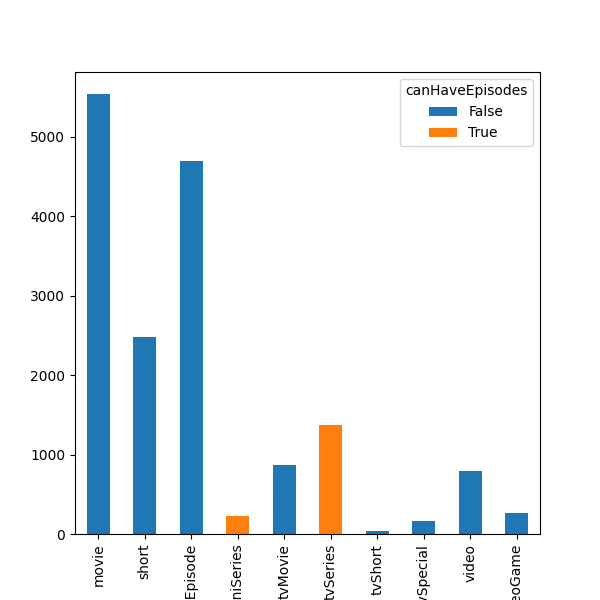
\includegraphics[width=0.45\textwidth]{plots/fig1_a.png} % Replace with your plot
        }
    \subfigure[(b)]{
        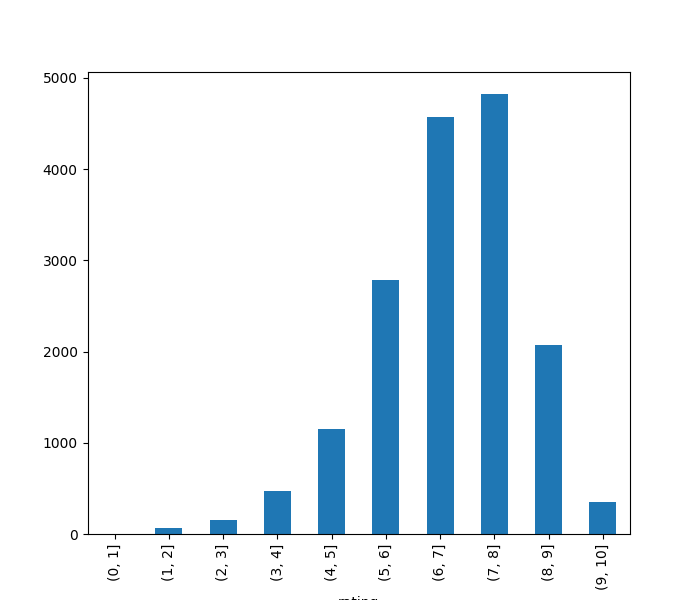
\includegraphics[width=0.45\textwidth]{plots/fig1_b.png}
        }
    \subfigure[(c)]{
        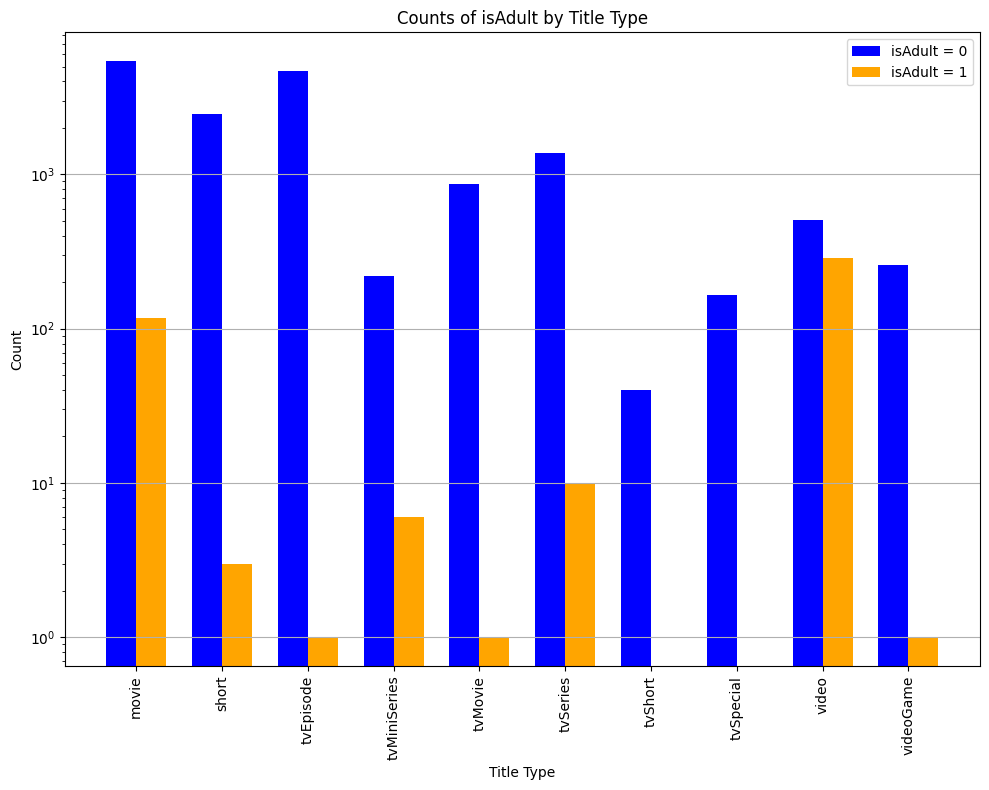
\includegraphics[width=0.45\textwidth]{plots/fig1_c.png}
        }
    \caption{Bar chart of the discrete attributes: (a): counting of the title types frequencies combined with the canHaveEpisodes variable (b): counting of ratings frequencies (c): counting of the adult and non-adult frequencies combined with the isRatable attribute.}
    \label{fig:bar-charts}
\end{figure}
\subsection{Continuous attributes}
...content...
...content...
...content...
...content...
...content...
...content...
...content...
...content...
...content...
...content...


\end{document}
